\documentclass[12pt,a4paper]{article}
\usepackage[utf8]{vietnam}
\usepackage{amsmath}
\usepackage{amsfonts}
\usepackage{amssymb}
\usepackage{graphicx}
\usepackage[left=3.5cm,right=2cm,top=2.5cm,bottom=2.5cm]{geometry}
\usepackage{graphicx}
\fontfamily{\ttdefault}  
\selectfont
\usepackage{fancyhdr}
\pagestyle{fancy}
\usepackage{multido}

\fancyhf{}
\renewcommand{\footrulewidth}{1pt}
\renewcommand*{\thesection}{\Alph{section}.}
\renewcommand*{\thesubsection}{\hspace{1cm}\Roman{subsection}.}
\renewcommand*{\thesubsubsection}{\hspace{1.5cm}\alph{subsubsection}.}
\setlength{\parindent}{1cm}
\lhead{SVTH: NGUYỄN THÀNH NHÂN}
\cfoot{\thepage}
\graphicspath{{D:/Báo cáo thực tập/pic}}

\newcommand{\Pointilles}[1]{%
  \par\nobreak
  \noindent\rule{0pt}{1.5\baselineskip} 
  \multido{}{#1}{\noindent\makebox[\linewidth]{\dotfill}\endgraf}
  \bigskip
}
\begin{document}
   \begin{center}
  {\Huge \textbf{LỜI MỞ ĐẦU }}
   \end{center}
   
Với nhu cầu sử dụng của con người ngày càng nhiều, để đáp lại điều đó khoa học - kỹ thuật đã phát triển rất nhiều nhằm đáp ứng nhu cầu ấy. Trong đó, sự phát triển mạnh nhất là ĐHKK, nó được sử dụng rộng rãi khắp mọi nơi như bệnh viện, văn phòng, trường học,...nó khiến người sử dụng thoải mái, mát mẻ và giúp họ đạt được kết quả tốt trong công việc.\\

Trong quá trình học tập tại nhà trường, em đã được trang bị và tích lũy rất nhiều kiến thức chuyên ngành bổ ích, nhưng để áp dụng kiến thức vào thực tế và làm cơ sở phục vụ cho việc làm luận văn tốt nghiệp, bản thân em và các bạn sinh viên khác đã được khoa và nhà trường tạo điều kiện hỗ trợ đi làm .Trong thời gian học tập và làm việc cùng các anh em kỹ sư , em được rất nhiều kinh nghiệm thực tế mà khi ngồi trên ghế nhà trường chưa được biết, đồng thời hiểu sâu hơn và định hướng về công việc mình sẽ đảm nhận sau này.\\

Em xin chân thành cảm ơn Ban lãnh đạo Công ty Cơ điện lạnh HACO cùng anh em kỹ thuật làm việc tại công trình đã tạo điều kiện, tận tình chỉ dẫn, cung cấp những kinh nghiệm thiết thực đã giúp em bổ sung cho mình những kiến thức thực tế, qua đó làm nền tảng cho công việc sau này. Em đã có một thời gian làm việc thật bổ ích tại công trình, được va chạm thực tế, tích lũy kiến thức cho bản thân.\\

Em xin cảm ơn nhà trường và thầy cô đã cho em kiến thức để có thể áp dụng vào thực tế và giúp em hiểu thêm về ngành mình đã chọn.\\

\newpage
\begin{center}
  {\Huge \textbf{GIỚI THIỆU CÔNG TY }}
\end{center}

\begin{enumerate}
   \item \textbf{Giới thiệu chung}
   
\hspace{1cm} Công ty TNHH Cơ điện lạnh HACO - (HACOME) được sáng lập 2018 hoạt động trên lĩnh vực cơ điện lạnh cho các công trình dân dụng.\\

\begin{figure}[htpb]
\centering
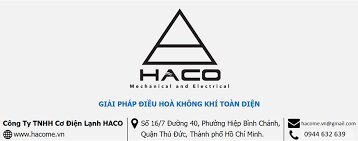
\includegraphics[scale=1]{haco}
\caption{HACOME}
\end{figure}

\hspace{1cm} Công ty TNHH cơ điện lạnh HACO là đại lý trực tiếp của DAIKIN, chuyên về tư vấn thiết kế, lắp đặt và phân phối, bảo trì...

\hspace{1cm} HACO đã đề ra sứ mệnh cung cấp giải pháp ĐHKK toàn diện, tiết kiếm với chất lượng phục vụ tốt, bằng đội ngũ kỹ thuật chuyên nghiệp tốt nhất thông qua các dòng sản phẩm tới từ đối tác uy tín trong ngành kỹ thuật điều hoà không khí - DAIKIN VRV, MULTI, SKYAIR, ROOMAIR, PACKAGED. Đồng thời HACO cũng đào tạo nghề nghiệp, phát triển con người...

\hspace{1cm} Nhằm phát triển ngày càng đi lên HACO đã đặt " TINH THẦN HACO " trong đó có 10 giá trị cốt lõi:
\begin{itemize}
 \item PHỤC VỤ: Luôn phục vụ khách hàng trên mức mong đợi.
 \item UY TÍN: Luôn giữ uy tín như giữ mạng.
 \item KẾT QUẢ: Luôn làm hết việc chứ không hết giờ.
 \item KẾ HOẠCH: Luôn làm việc có kế hoạch.
 \item ĐỒNG ĐỘI: Luôn sẵn sàng giúp đỡ đồng đội.
 \item TÍCH CỰC: Luôn suy nghĩ tích cực và đơn giản hoá.
 \item CHỦ ĐỘNG: Luôn chủ động trong công việc.
 \item TRÁCH NHIỆM: Luôn chịu trách nhiệm 100%.
 \item GIẢI PHÁP: Luôn tìm giải pháp để đạt mục tiêu.
 \item TÌNH YÊU: Luôn yêu công việc mình làm.
\end{itemize}

\newpage
\item \textbf{HỒ SƠ CÔNG TY.}

\hspace{1cm} - Giấy phép kinh doanh ( MS Thuế ): 0315854277 - ngày cấp: 17/0820/19.

\hspace{1cm} - Tên công ty: CÔNG TY TNHH CƠ ĐIỆN LẠNH HACO.

\hspace{1cm} - Tên giao dịch: HACOME CO., LTD.

\hspace{1cm} - Chủ tịch ( Đại diện pháp luật ): Đoàn Thị Kim Nhung.

\hspace{1cm} - Loại hình hoạt động: Công ty TNHH.

\hspace{1cm} - Thị trường hoạt động: VIỆT NAM.

\hspace{1cm} - Số lượng nhân viên: 15 - 20 nhân viên.

\item \textbf{THÔNG TIN LIÊN LẠC.}

\hspace{1cm} - Địa chỉ trụ sở chính: 16/7 đường số 40, phường Hiệp Bình Chánh, quận Thủ Đức, Tp.HCM.

\hspace{1cm} - Điện thoại: 0944 632 639.

\hspace{1cm} - Email: hacome.vn@gmail.com


\item \textbf{DỰ ÁN TIÊU BIỂU}

\begin{enumerate}
\item \textbf{VẠN PHÚC CITY - THỦ ĐỨC, TP.HCM.}
\begin{figure}[htbp]
  \centering
  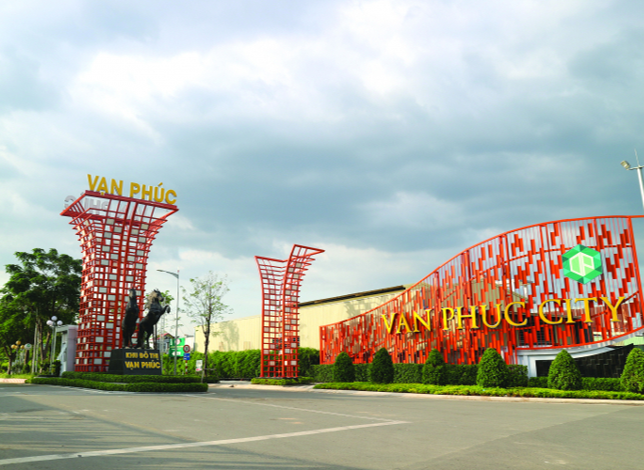
\includegraphics[scale=0.6]{van phuc city}
  \caption{VẠN PHÚC CITY}
\end{figure}

\hspace{1cm} - Chủ đầu tư: Ms. Loan.

\hspace{1cm} - Thi công: Công ty TNHH HACOME.

\hspace{1cm} - Địa chỉ: Số 1 đường số 1.

\hspace{1cm} - Thiết bị DAIKIN: VRV.

\hspace{1cm} - Năm hoàn thành: 2019.

\item \textbf{VILLA LAGI - TP. PHAN THIẾT.}
\begin{figure}[htbp]
  \centering
  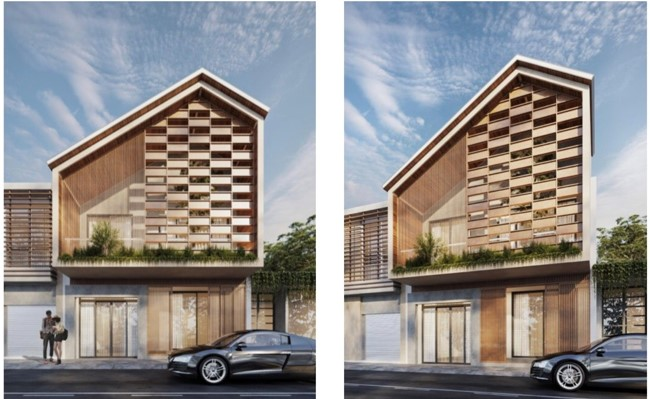
\includegraphics[scale=0.8]{lagi phan thiet}
  \caption{VILLA LAGI PHAN THIẾT}
\end{figure}

\hspace{1cm} - Chủ đầu tư: Mr. Dũng.

\hspace{1cm} - Thi công: Công ty TNHH HACOME.

\hspace{1cm} - Địa chỉ: Số 1 Thống Nhất, P. Phước Hội, TX. Lagi.

\hspace{1cm} - Thiết bị DAIKIN: VRV - Giấu trần nối ống gió.

\hspace{1cm} - Năm hoàn thành: 2020.

\item \textbf{VILLA VEROSA PARK - QUẬN 9, TP.HCM.}
\begin{figure}[htbp]
  \centering
  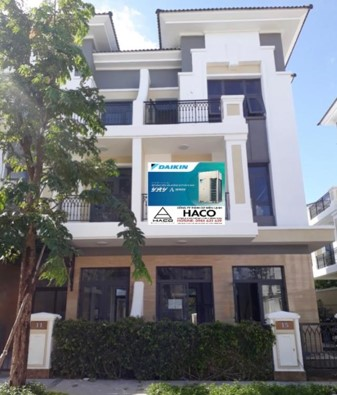
\includegraphics[scale=0.6]{verosa park}
  \caption{VILLA VEROSA PARK}
\end{figure}
\newpage
\hspace{1cm} - Chủ đầu tư: Ms. Nhi.

\hspace{1cm} - Thi công: Công ty TNHH HACOME.

\hspace{1cm} - VEROSA PARK, Khang Điền, Q.9, Tp.HCM.

\hspace{1cm} - Thiết bị DAIKIN: VRV - Giấu trần nối ống gió.

\hspace{1cm} - Năm hoàn thành: 2020.

\item \textbf{SHOWROOM ĐẠI PHÚ QUÍ - BIÊN HOÀ ĐỒNG NAI, TP.HCM.}
\begin{figure}[htbp]
  \centering
  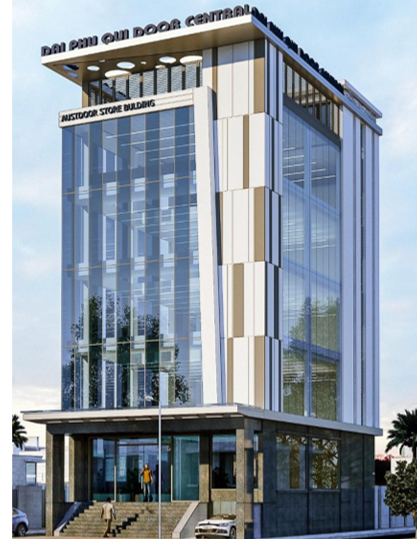
\includegraphics[scale=1]{dai phu quy}
  \caption{SHOWROOM ĐẠI PHÚ QUÍ}
\end{figure}

\hspace{1cm} - Chủ đầu tư: Mr. Qúi.

\hspace{1cm} - Thi công: Công ty TNHH HACOME.

\hspace{1cm} - Biên Hoà, Đồng Nai.

\hspace{1cm} - Thiết bị DAIKIN: VRV A - Giấu trần nối ống gió.

\hspace{1cm} - Năm hoàn thành: 2020.

\newpage
\item \textbf{VĂN PHÒNG LÀM VIỆC - KHU CÔNG NGHIỆP\\
 LONG GIANG.}
\begin{figure}[htbp]
  \centering
  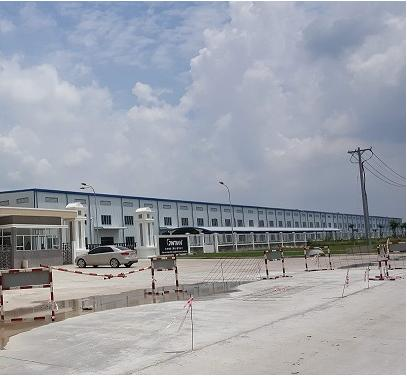
\includegraphics[scale=0.6]{long giang}
  \caption{VĂN PHÒNG LÀM VIỆC LONG GIANG}
\end{figure}

\hspace{1cm} - Chủ đầu tư: Mr. Kiên.

\hspace{1cm} - Thi công: Công ty TNHH HACOME.

\hspace{1cm} - Khu công nghiệp Long Giang, Mỹ Tho - Tiền Giang.

\hspace{1cm} - Thiết bị DAIKIN: VRV A - Cassette âm trần đa hướng thổi.

\hspace{1cm} - Năm hoàn thành: 2020.
\end{enumerate}

\newpage
\item \textbf{NỘI DUNG THỰC TẬP}

1. Nhân viên văn phòng:

\hspace{1cm} - Tìm hiểu về các nhà cung cấp vật tư.

\hspace{1cm} - Liệt kê các vật tư cần đặt hàng.

\hspace{1cm} - Gửi khối lượng để lấy báo giá.

\hspace{1cm} - Đặt hàng để thi công.
	
\begin{figure}[htbp]
  \centering
  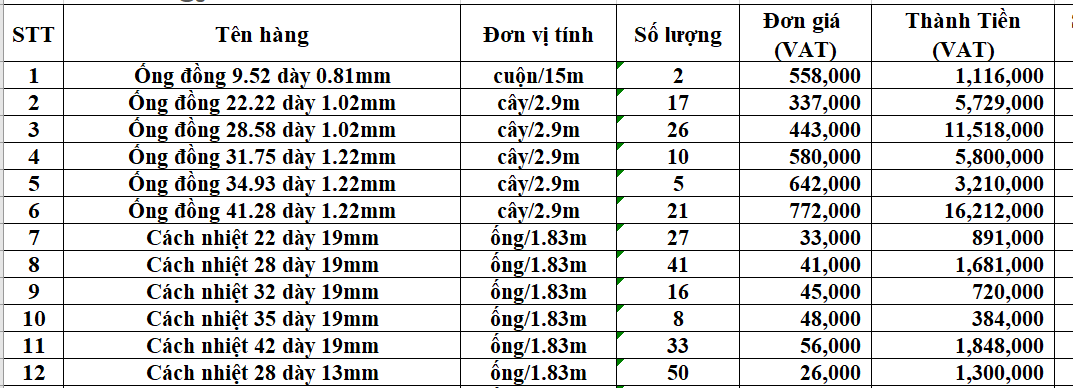
\includegraphics[scale=0.7]{bao gia}
  \caption{BÁO GIÁ KHỐI LƯỢNG MR. KIÊN }
\end{figure}

2. Nhân viên kỹ thuật:

\hspace{1cm} - Tham gia các công việc bảo trì và vệ sinh máy
\begin{figure}[htbp]
  \centering
  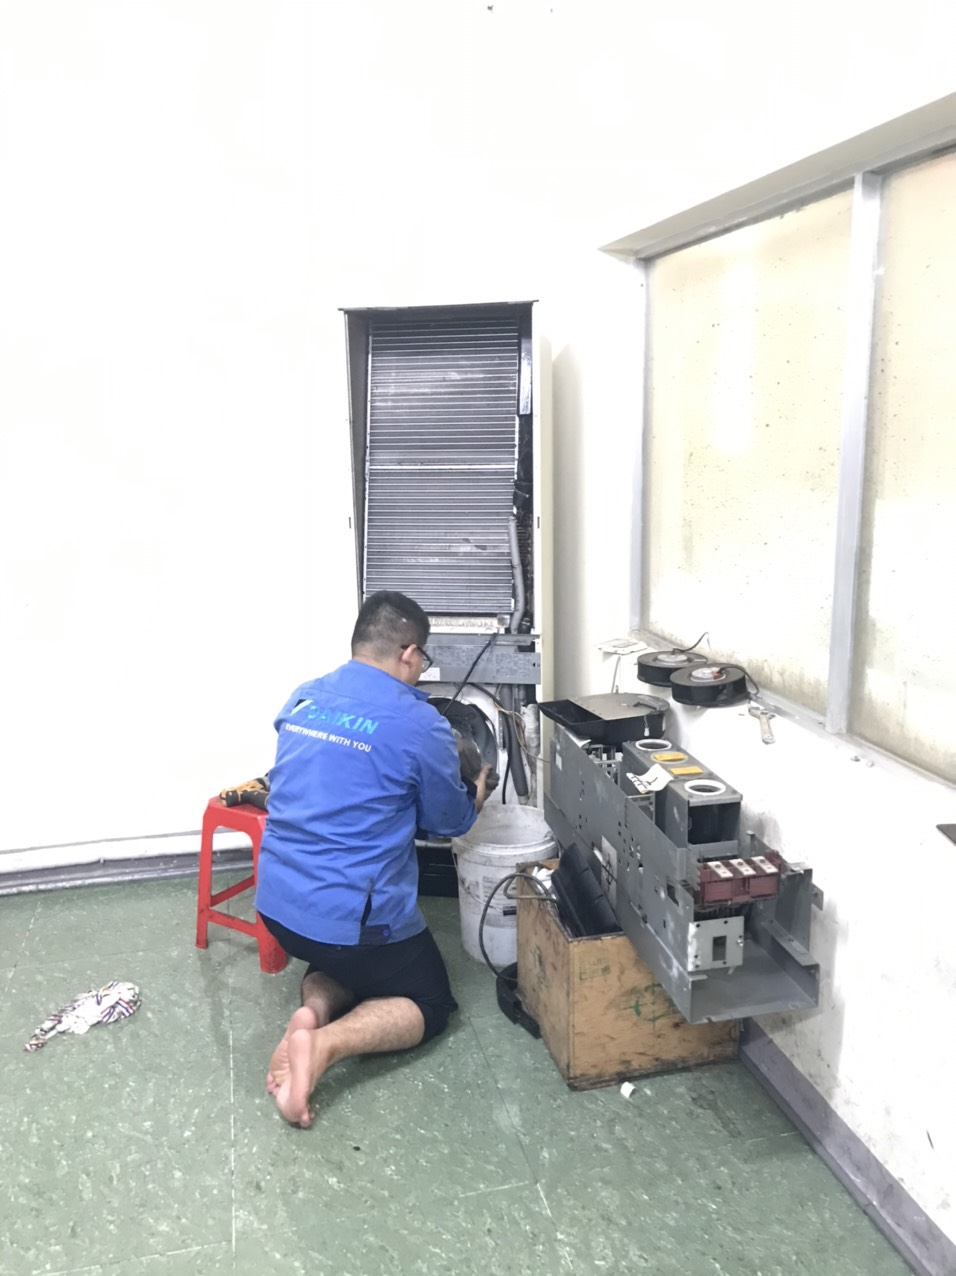
\includegraphics[scale=0.2]{bao tri}
  \caption{BẢO TRÌ SUNSTEEL }
\end{figure}

\newpage
\hspace{1cm} - Tham gia kết nối ống đồng, lắp đặt, kết nối ống gió, kết nối box gió...
\begin{figure}[htbp]
  \centering
  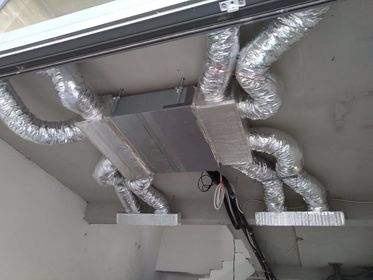
\includegraphics[scale=0.6]{ket noi}
  \caption{KẾT NỐI ỐNG ĐỒNG, ỐNG GIÓ }
\end{figure}
\end{enumerate}

\newpage
\begin{center}
  {\Huge \textbf{NHẬN XÉT }}
\end{center}
\Pointilles{44}

\end{document}